\documentclass[tikz,border=5pt]{standalone}
\usetikzlibrary{calc,positioning,intersections,shadows.blur,decorations.pathmorphing,patterns,shapes.callouts}

\definecolor{moonGray}{RGB}{180,180,180}
\definecolor{craterGray}{RGB}{120,120,120}
\definecolor{spaceBlue}{RGB}{10,10,40}
\definecolor{sunlight}{RGB}{255, 215, 0}
\definecolor{earthBlue}{RGB}{60,170,255}
\definecolor{earthGreen}{RGB}{40,140,60}
\definecolor{bedrock}{RGB}{120, 120, 120}
\definecolor{regolith}{RGB}{180, 150, 120}

\begin{document}
\begin{tikzpicture}[scale=1.2]

% White background for the entire area with equal borders
\fill[white] (-0,-4.1) rectangle (13.1,3.5);

% Three separate space boxes above each surface section with larger boxes
\fill[spaceBlue] (0,0) rectangle (4,3.5);
\fill[spaceBlue] (4.5,0) rectangle (8.5,3.5);
\fill[spaceBlue] (9,0) rectangle (13,3.5);

% Add stars to each space section
\foreach \i in {1,...,25}{
  \fill[white] (rnd*4,rnd*2+1.2) circle (0.02);
}
\foreach \i in {1,...,25}{
  \fill[white] (4.5+rnd*4,rnd*2+1.2) circle (0.02);
}
\foreach \i in {1,...,25}{
  \fill[white] (9+rnd*4,rnd*2+1.2) circle (0.02);
}

% Day case section (left) - larger
\shade[top color=regolith, bottom color=bedrock] (0,-2.5) rectangle (4,0);
\fill[bedrock] (0,-4) rectangle (4,-2.4);

% Night case section (middle) - larger
\shade[top color=regolith, bottom color=bedrock] (4.5,-2.5) rectangle (8.5,0);
\fill[bedrock] (4.5,-4) rectangle (8.5,-2.4);

% Eclipse case section (right) - larger
\shade[top color=regolith, bottom color=bedrock] (9,-2.5) rectangle (13,0);
\fill[bedrock] (9,-4) rectangle (13,-2.4);

% Add rock fragments randomly distributed in each section - same pattern for all
\pgfmathsetseed{42} % Set seed for reproducible randomness
\foreach \i in {1,...,10} {
    \pgfmathsetmacro{\xrel}{rnd*3}
    \pgfmathsetmacro{\y}{-0.3 + rnd*(-2.2)}
    \pgfmathsetmacro{\size}{0.1 + rnd*0.15}
    
    % Day case section
    \fill[bedrock] (\xrel,\y) -- (\xrel+\size,\y-0.05) -- (\xrel+\size+0.05,\y+\size*0.7) -- (\xrel+\size*0.5,\y+\size) -- (\xrel,\y+\size*0.5) -- cycle;
    
    % Night case section
    \pgfmathsetmacro{\xnight}{4.5 + \xrel}
    \fill[bedrock] (\xnight,\y) -- (\xnight+\size,\y-0.05) -- (\xnight+\size+0.05,\y+\size*0.7) -- (\xnight+\size*0.5,\y+\size) -- (\xnight,\y+\size*0.5) -- cycle;
    
    % Eclipse case section
    \pgfmathsetmacro{\xeclipse}{9 + \xrel}
    \fill[bedrock] (\xeclipse,\y) -- (\xeclipse+\size,\y-0.05) -- (\xeclipse+\size+0.05,\y+\size*0.7) -- (\xeclipse+\size*0.5,\y+\size) -- (\xeclipse,\y+\size*0.5) -- cycle;
}

% Textured surface lines for each section
\draw[black,thick,decorate,decoration={random steps, segment length=3pt, amplitude=0.8pt}] (0,0) -- (4,0);
\draw[black,thick,decorate,decoration={random steps, segment length=3pt, amplitude=0.8pt}] (4.5,0) -- (8.5,0);
\draw[black,thick,decorate,decoration={random steps, segment length=3pt, amplitude=0.8pt}] (9,0) -- (13,0);

% Labels for each case
\node[white,anchor=center,font=\Large\bfseries] at (2,3) {DAY};
\node[white,anchor=center,font=\Large\bfseries] at (6.5,3) {NIGHT};
\node[white,anchor=center,font=\Large\bfseries] at (11,3) {ECLIPSE};

% Add grey dotted lines at turning points with improved labels and positioning
% 10e-1 depth (top line)
\draw[gray!60!black, very thick, dotted] (0.0,-2.3) -- (4.0,-2.3);
\draw[gray!60!black, very thick, dotted] (4.5,-2.3) -- (8.5,-2.3);
\draw[gray!60!black, very thick, dotted] (9.0,-2.3) -- (13.0,-2.3);
\node[black, anchor=east, font=\footnotesize] at (0.0,-2.3) {$10^{-1}$};

% 10e-2 depth (middle line)
\draw[gray!60!black, very thick, dotted] (0.0,-1.0) -- (4.0,-1.0);
\draw[gray!60!black, very thick, dotted] (4.5,-1.0) -- (8.5,-1.0);
\draw[gray!60!black, very thick, dotted] (9.0,-1.0) -- (13.0,-1.0);
\node[black, anchor=east, font=\footnotesize] at (0.0,-1.0) {$10^{-2}$};

% Surface label (10^-3)
\node[black, anchor=east, font=\footnotesize] at (0.0,-0.2) {$10^{-3}$};

% Bottom label (10^0)
\node[black, anchor=east, font=\footnotesize] at (0.0,-3.9) {$10^{0}$};

% Depth axis label on the left side
\node[black, anchor=center, font=\small\bfseries, rotate=90] at (-0.9,-1.8) {Depth [m]};

% Temperature axis label on the bottom
\node[black, anchor=center, font=\small\bfseries] at (6.5,-4.5) {Temperature [K]};

% Ticklabels
\node[black, anchor=north, font=\footnotesize] at (0.0,-4.0) {$100$};
\node[black, anchor=north, font=\footnotesize] at (2.0,-4.0) {$250$};
\node[black, anchor=north, font=\footnotesize] at (4.0,-4.0) {$400$};
\node[black, anchor=north, font=\footnotesize] at (4.5,-4.0) {$100$};
\node[black, anchor=north, font=\footnotesize] at (6.5,-4.0) {$250$};
\node[black, anchor=north, font=\footnotesize] at (8.5,-4.0) {$400$};
\node[black, anchor=north, font=\footnotesize] at (9.0,-4.0) {$100$};
\node[black, anchor=north, font=\footnotesize] at (11.0,-4.0) {$250$};
\node[black, anchor=north, font=\footnotesize] at (13.0,-4.0) {$400$};

% Temperature-depth profiles based on realistic lunar data
% Day case - surface heating with exponential decay
\begin{scope}
\draw[blue, very thick] plot[smooth] coordinates {
  (3.8,0) (3.6,-1.0) (2.5,-1.75) (2.0,-2.0) (1.8,-2.3) (2.0,-2.8) (1.9,-4.0)
};
\end{scope}

% Night case - cooling from surface
\begin{scope}[xshift=4.5cm]
\draw[blue, very thick] plot[smooth] coordinates {
  (0.2,0) (0.7,-1.2) (1.5,-2.0) (2.2,-2.5) (2.0,-3.2) (1.9,-4.0)
};
\end{scope}

% Eclipse case - similar to night but with different surface temperature
\begin{scope}[xshift=9.0cm]
\draw[blue, very thick] plot[smooth] coordinates {
  (1.4,0) (3.2,-1.0) (2.5,-1.75) (2.0,-2.1) (1.8,-2.3) (1.8,-2.5) (2.0,-3.0) (1.9,-4.0)
};
\end{scope}

% Solar rays hitting the day case (left section)
\foreach \i in {0,...,5} {
    \draw[sunlight,thick,->] (0.2 + \i*0.2, 3.5) -- (1.5 + \i*0.2, 0);
}

% Eclipse case rays - same angle as day case but shifted to eclipse section and blocked by Earth
\foreach \i in {0,...,5} {
    \draw[sunlight,thick,->] (9.2 + \i*0.2, 3.5) -- (9.9 + \i*0.2, 1.8);
}

% Enhanced Earth positioned to block the eclipse rays
\begin{scope}[xshift=-0.14cm, yshift=-0.45cm]
% Atmosphere glow
\shade[inner color=earthBlue!30, outer color=earthBlue!5] (10.5,2.3) circle (1.1*0.5);

% Main Earth body
\shade[ball color=earthBlue, shading angle=120] (10.5,2.3) circle (0.5);

% Enhanced continents
\clip (10.5,2.3) circle (0.5);
\fill[earthGreen!90] ($(10.5,2.3)+(-0.16,0.10)$) 
    .. controls +(0.35,0.15) and +(-0.25,-0.10) .. ($(10.5,2.3)+(0.30,0.15)$)
    .. controls +(-0.15,0.10) and +(0.10,0.15) .. ($(10.5,2.3)+(0.05,-0.05)$)
    .. controls +(-0.25,-0.15) and +(0.20,-0.10) .. cycle;

\fill[earthGreen!90] ($(10.5,2.3)+(-0.30,-0.08)$) 
    .. controls +(0.20,-0.15) and +(-0.15,0.15) .. ($(10.5,2.3)+(-0.05,-0.20)$)
    .. controls +(0.15,0.10) and +(-0.20,0.15) .. ($(10.5,2.3)+(-0.20,0.03)$) -- cycle;
    
% Cloud patterns
\fill[white,opacity=0.3] ($(10.5,2.3)+(-0.05,0.20)$) 
    .. controls +(0.15,0) and +(-0.10,0.05) .. ($(10.5,2.3)+(0.20,0.10)$)
    .. controls +(0,0.05) and +(0.10,0) .. ($(10.5,2.3)+(0.10,0.25)$)
    .. controls +(-0.10,0) and +(0.05,-0.05) .. cycle;

\draw[thick,earthBlue!80] (10.5,2.3) circle (0.5);
\end{scope}

% Red wavy arrows emitted from surface upwards (thermal radiation)
% Day case
\foreach \i in {0,...,3} {
    \draw[red,thick,->,decorate,decoration={snake, segment length=6pt, amplitude=2pt}] (0.8 + \i*0.8, 0) -- (0.8 + \i*0.8, 0.8);
}

% Night case
\foreach \i in {0,...,3} {
    \draw[red,thick,->,decorate,decoration={snake, segment length=6pt, amplitude=2pt}] (5.3 + \i*0.8, 0) -- (5.3 + \i*0.8, 0.4);
}

% Eclipse case
\foreach \i in {0,...,3} {
    \draw[red,thick,->,decorate,decoration={snake, segment length=6pt, amplitude=2pt}] (9.8 + \i*0.8, 0) -- (9.8 + \i*0.8, 0.6);
}

% Add LRO image in top right corner of each section
\node[anchor=north east] at (3.8,3.3) {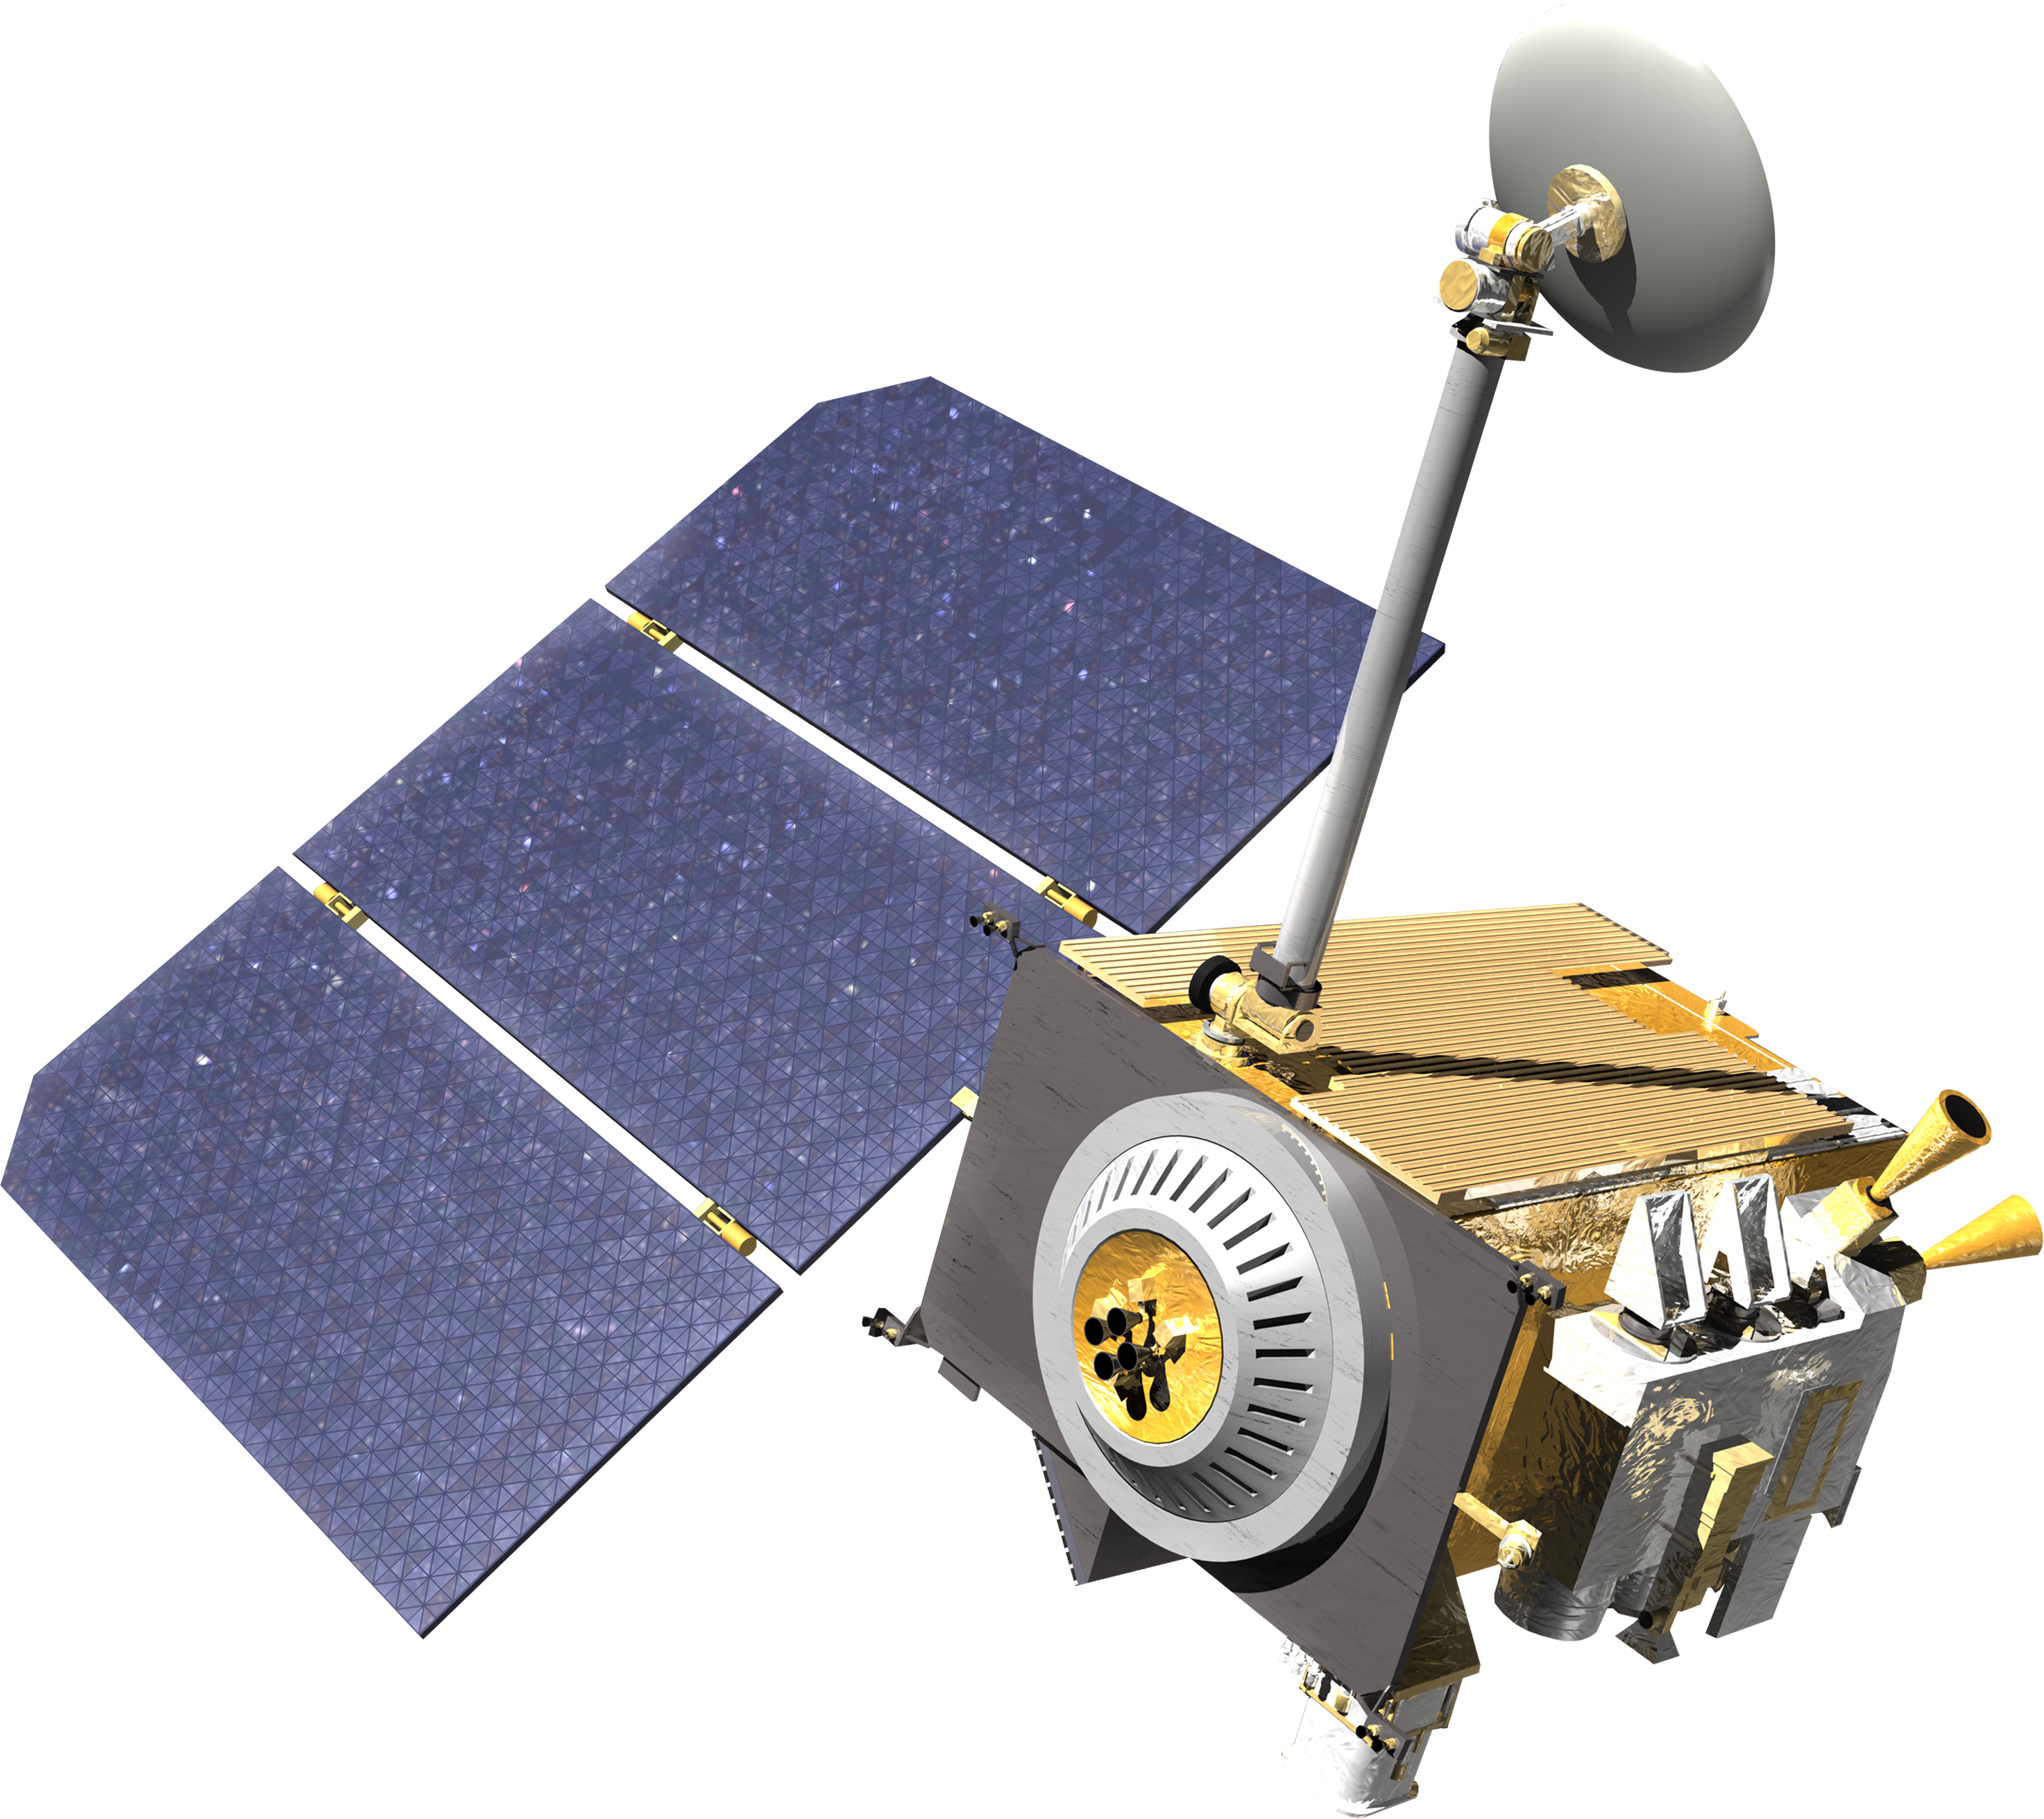
\includegraphics[width=0.8cm]{textures/LRO.png}};
\node[anchor=north east] at (8.3,3.3) {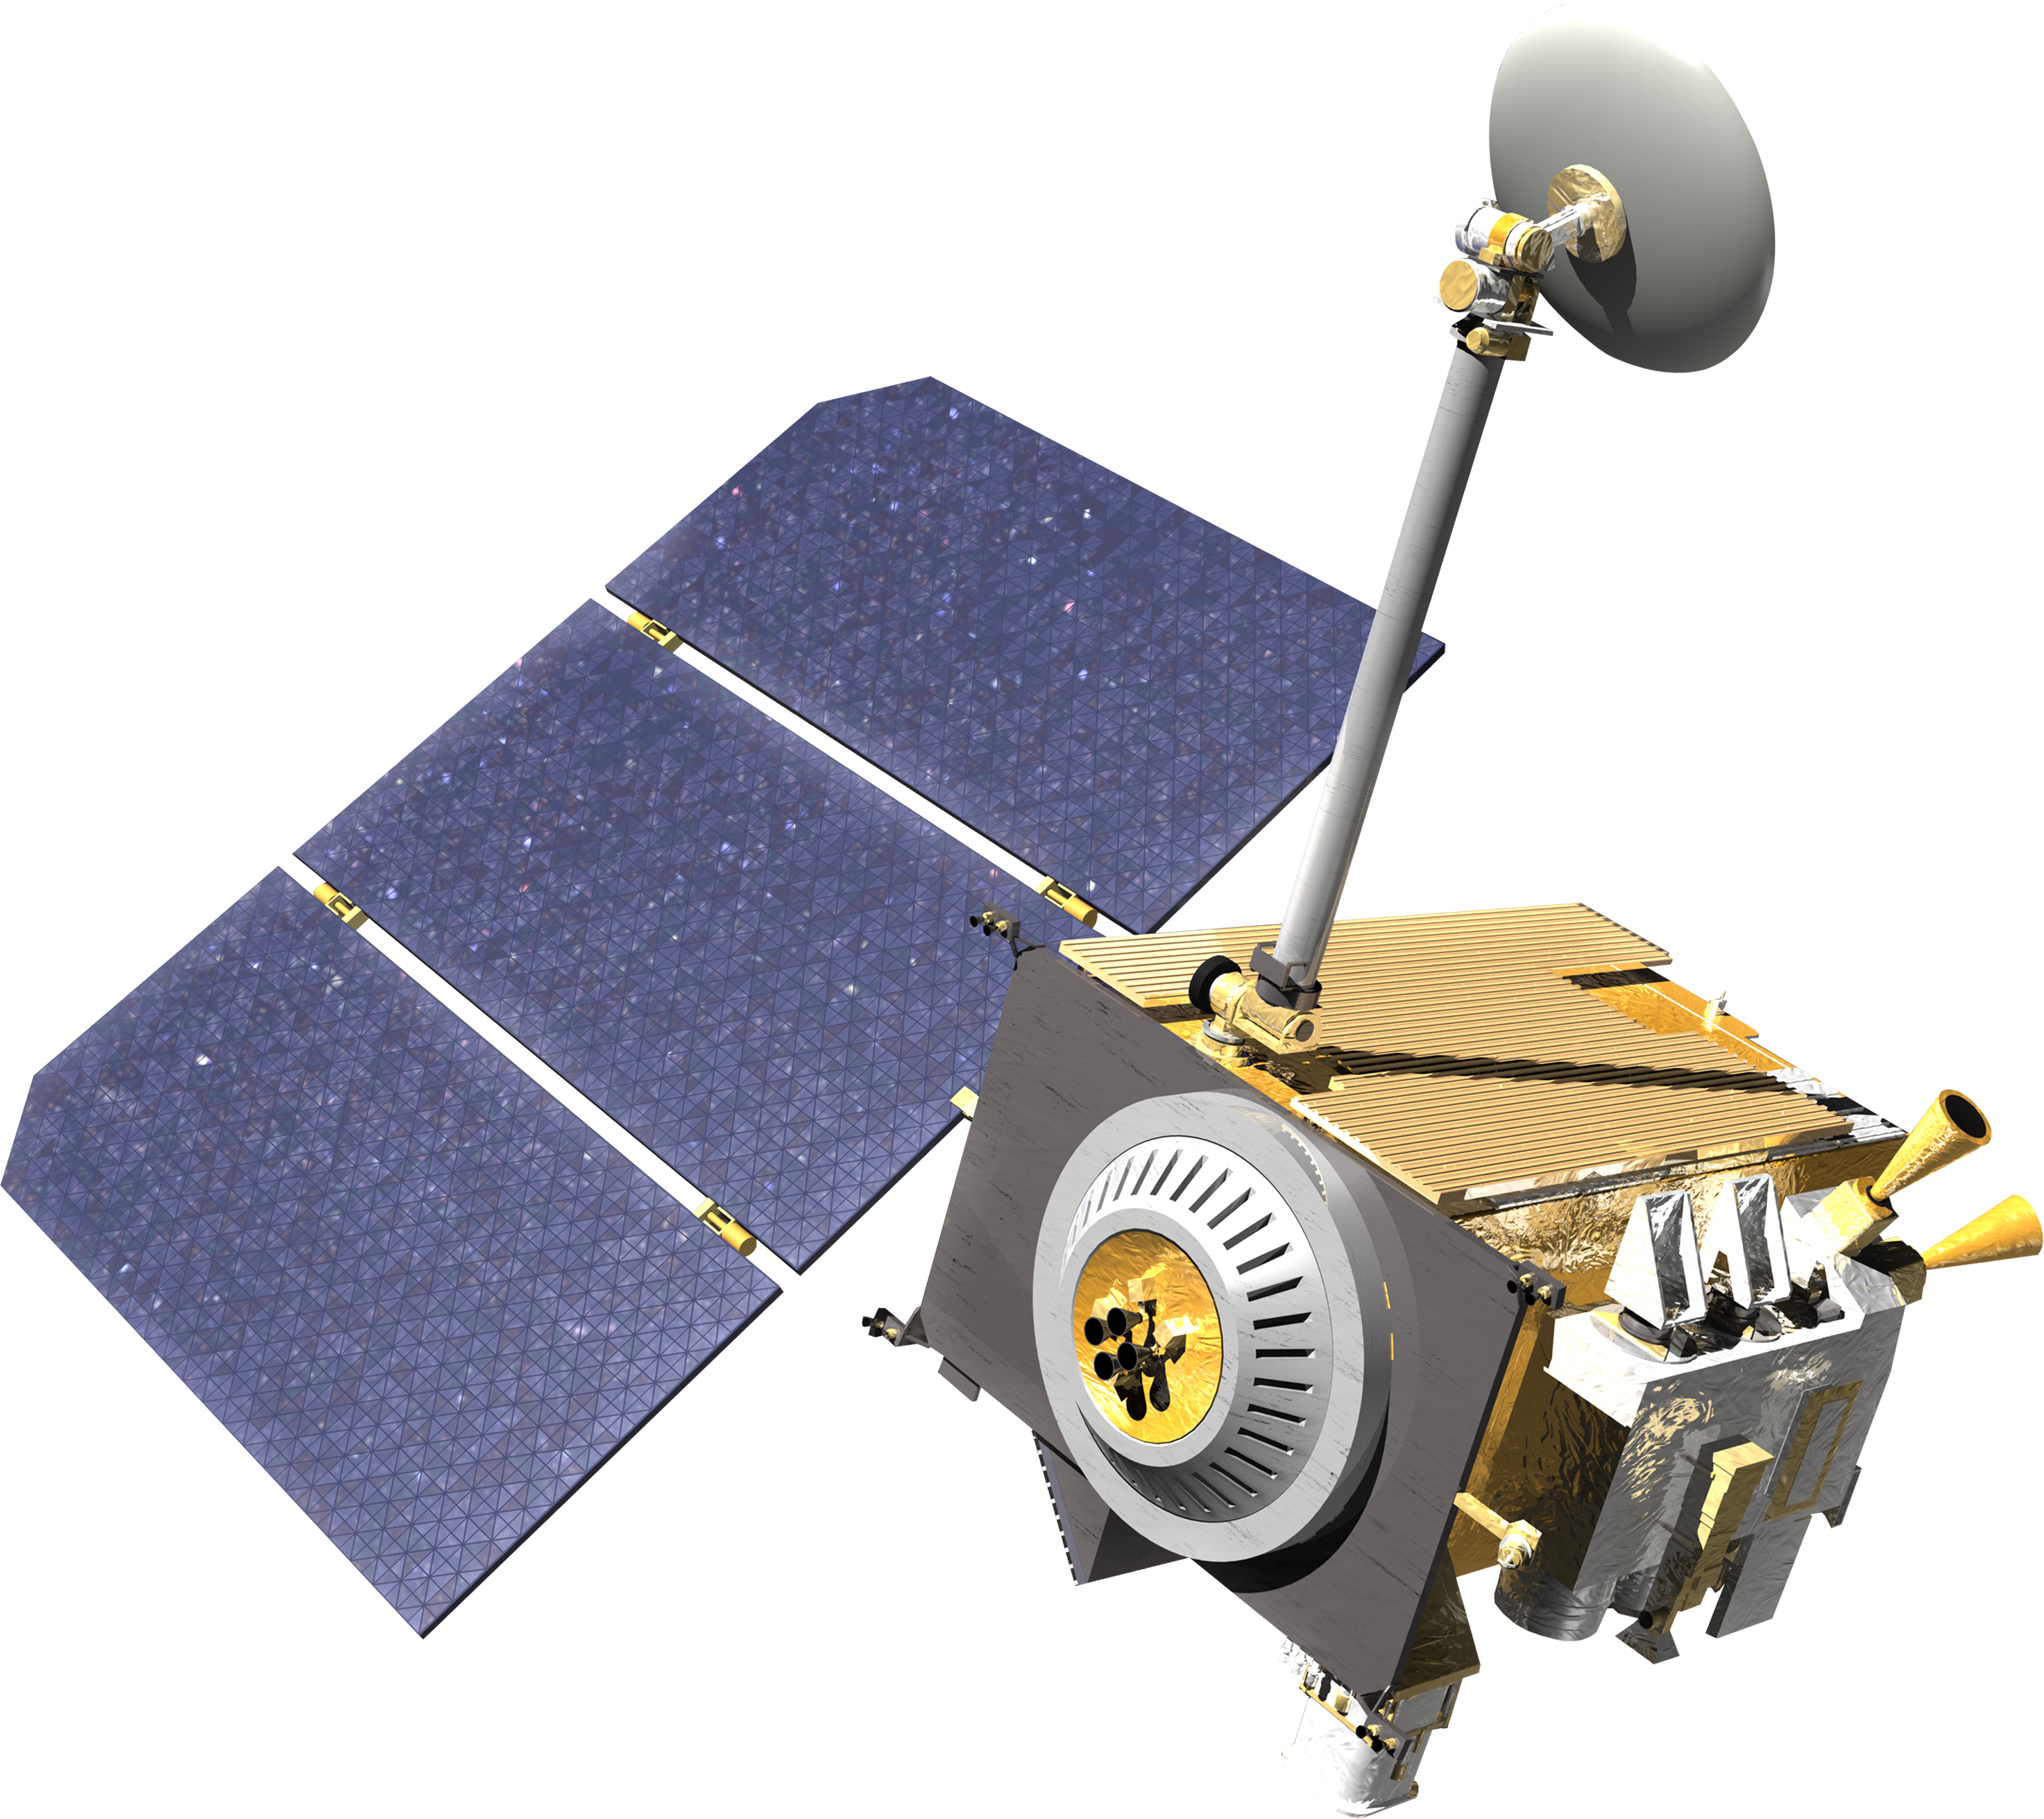
\includegraphics[width=0.8cm]{textures/LRO.png}};
\node[anchor=north east] at (12.8,3.3) {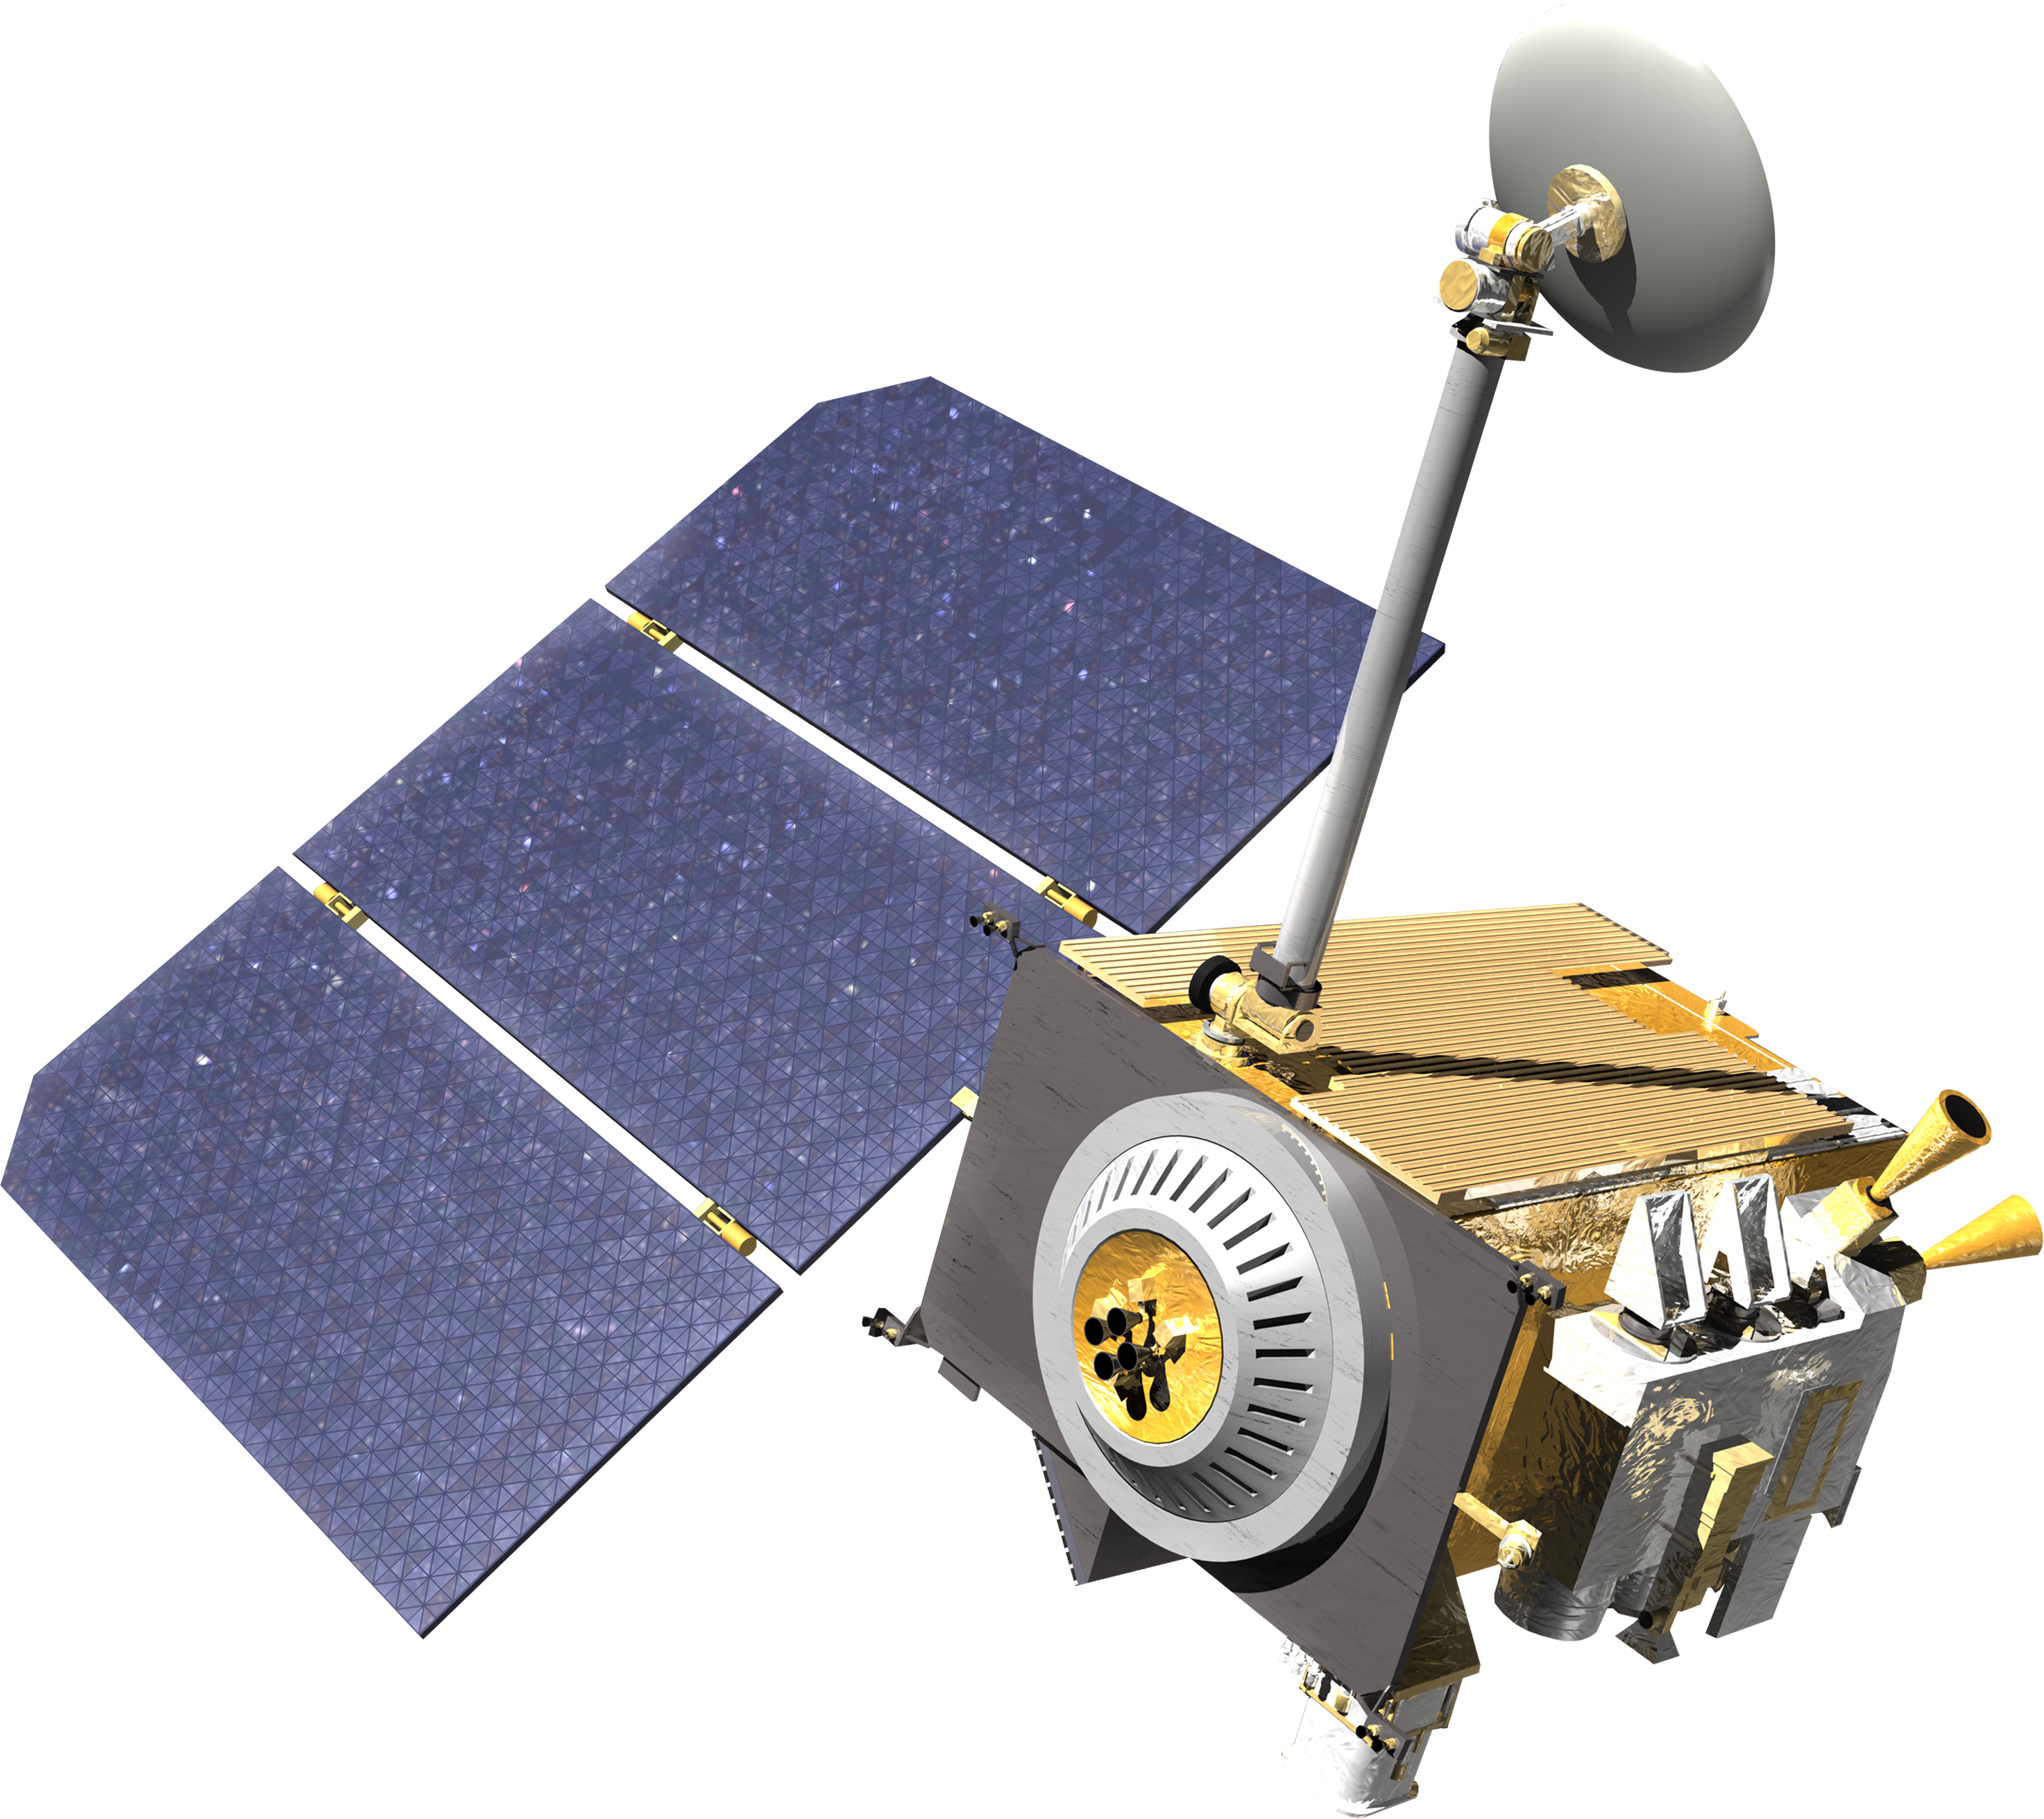
\includegraphics[width=0.8cm]{textures/LRO.png}};

% Add triangular FOV scan beams from LRO
% Day case FOV
\draw[yellow, thick, opacity=0.7] (3.4,2.7) -- (2.8,0) -- (3.2,0) -- cycle;
\draw[yellow, thick, opacity=0.7] (3.4,2.7) -- (3.2,0) -- (3.6,0) -- cycle;

% Night case FOV  
\draw[yellow, thick, opacity=0.7] (7.9,2.7) -- (7.3,0) -- (7.7,0) -- cycle;
\draw[yellow, thick, opacity=0.7] (7.9,2.7) -- (7.7,0) -- (8.1,0) -- cycle;

% Eclipse case FOV
\draw[yellow, thick, opacity=0.7] (12.4,2.7) -- (11.8,0) -- (12.2,0) -- cycle;
\draw[yellow, thick, opacity=0.7] (12.4,2.7) -- (12.2,0) -- (12.6,0) -- cycle;

\end{tikzpicture}
\end{document}